% ============================================================================================
% BAB III ANALISIS MASALAH
% Pembagian subbab tidak rigid dan dapat bervariasi. Bab ini minimal berisi analisis kebutuhan
% fungsional dan nonfungsional, analisis berbagai alternatif solusi yang dapat ditawarkan, dan
% metode pemilihan solusi yang diusulkan.
% ============================================================================================
\chapter{ANALISIS MASALAH}
\label{chap:analisis-masalah}

Bab ini menyajikan analisis mendalam terhadap kondisi sistem komunitas Telegram Michael Yeoh saat ini, identifikasi masalah spesifik yang dihadapi, analisis kebutuhan sistem rangkuman otomatis, serta evaluasi berbagai alternatif solusi dengan justifikasi pemilihan pendekatan yang diusulkan. Analisis ini menjadi fondasi untuk desain konsep solusi yang akan diuraikan pada Bab \ref{chap:desain-konsep-solusi}.

% ==========================================
\section{Analisis Kondisi Saat Ini}
\label{sec:kondisi-saat-ini}

\subsection{Model Konseptual Komunitas Telegram Eksisting}

Komunitas investasi saham Indonesia Michael Yeoh di Telegram merupakan ekosistem informasi finansial berskala besar dengan struktur hierarkis empat tingkat yang dirancang untuk menyediakan nilai berbeda pada setiap level keanggotaan. Gambar \ref{fig:current-system} mengilustrasikan arsitektur sistem komunikasi komunitas saat ini beserta aliran informasi antar komponen.

\begin{figure}[H]
  \centering
  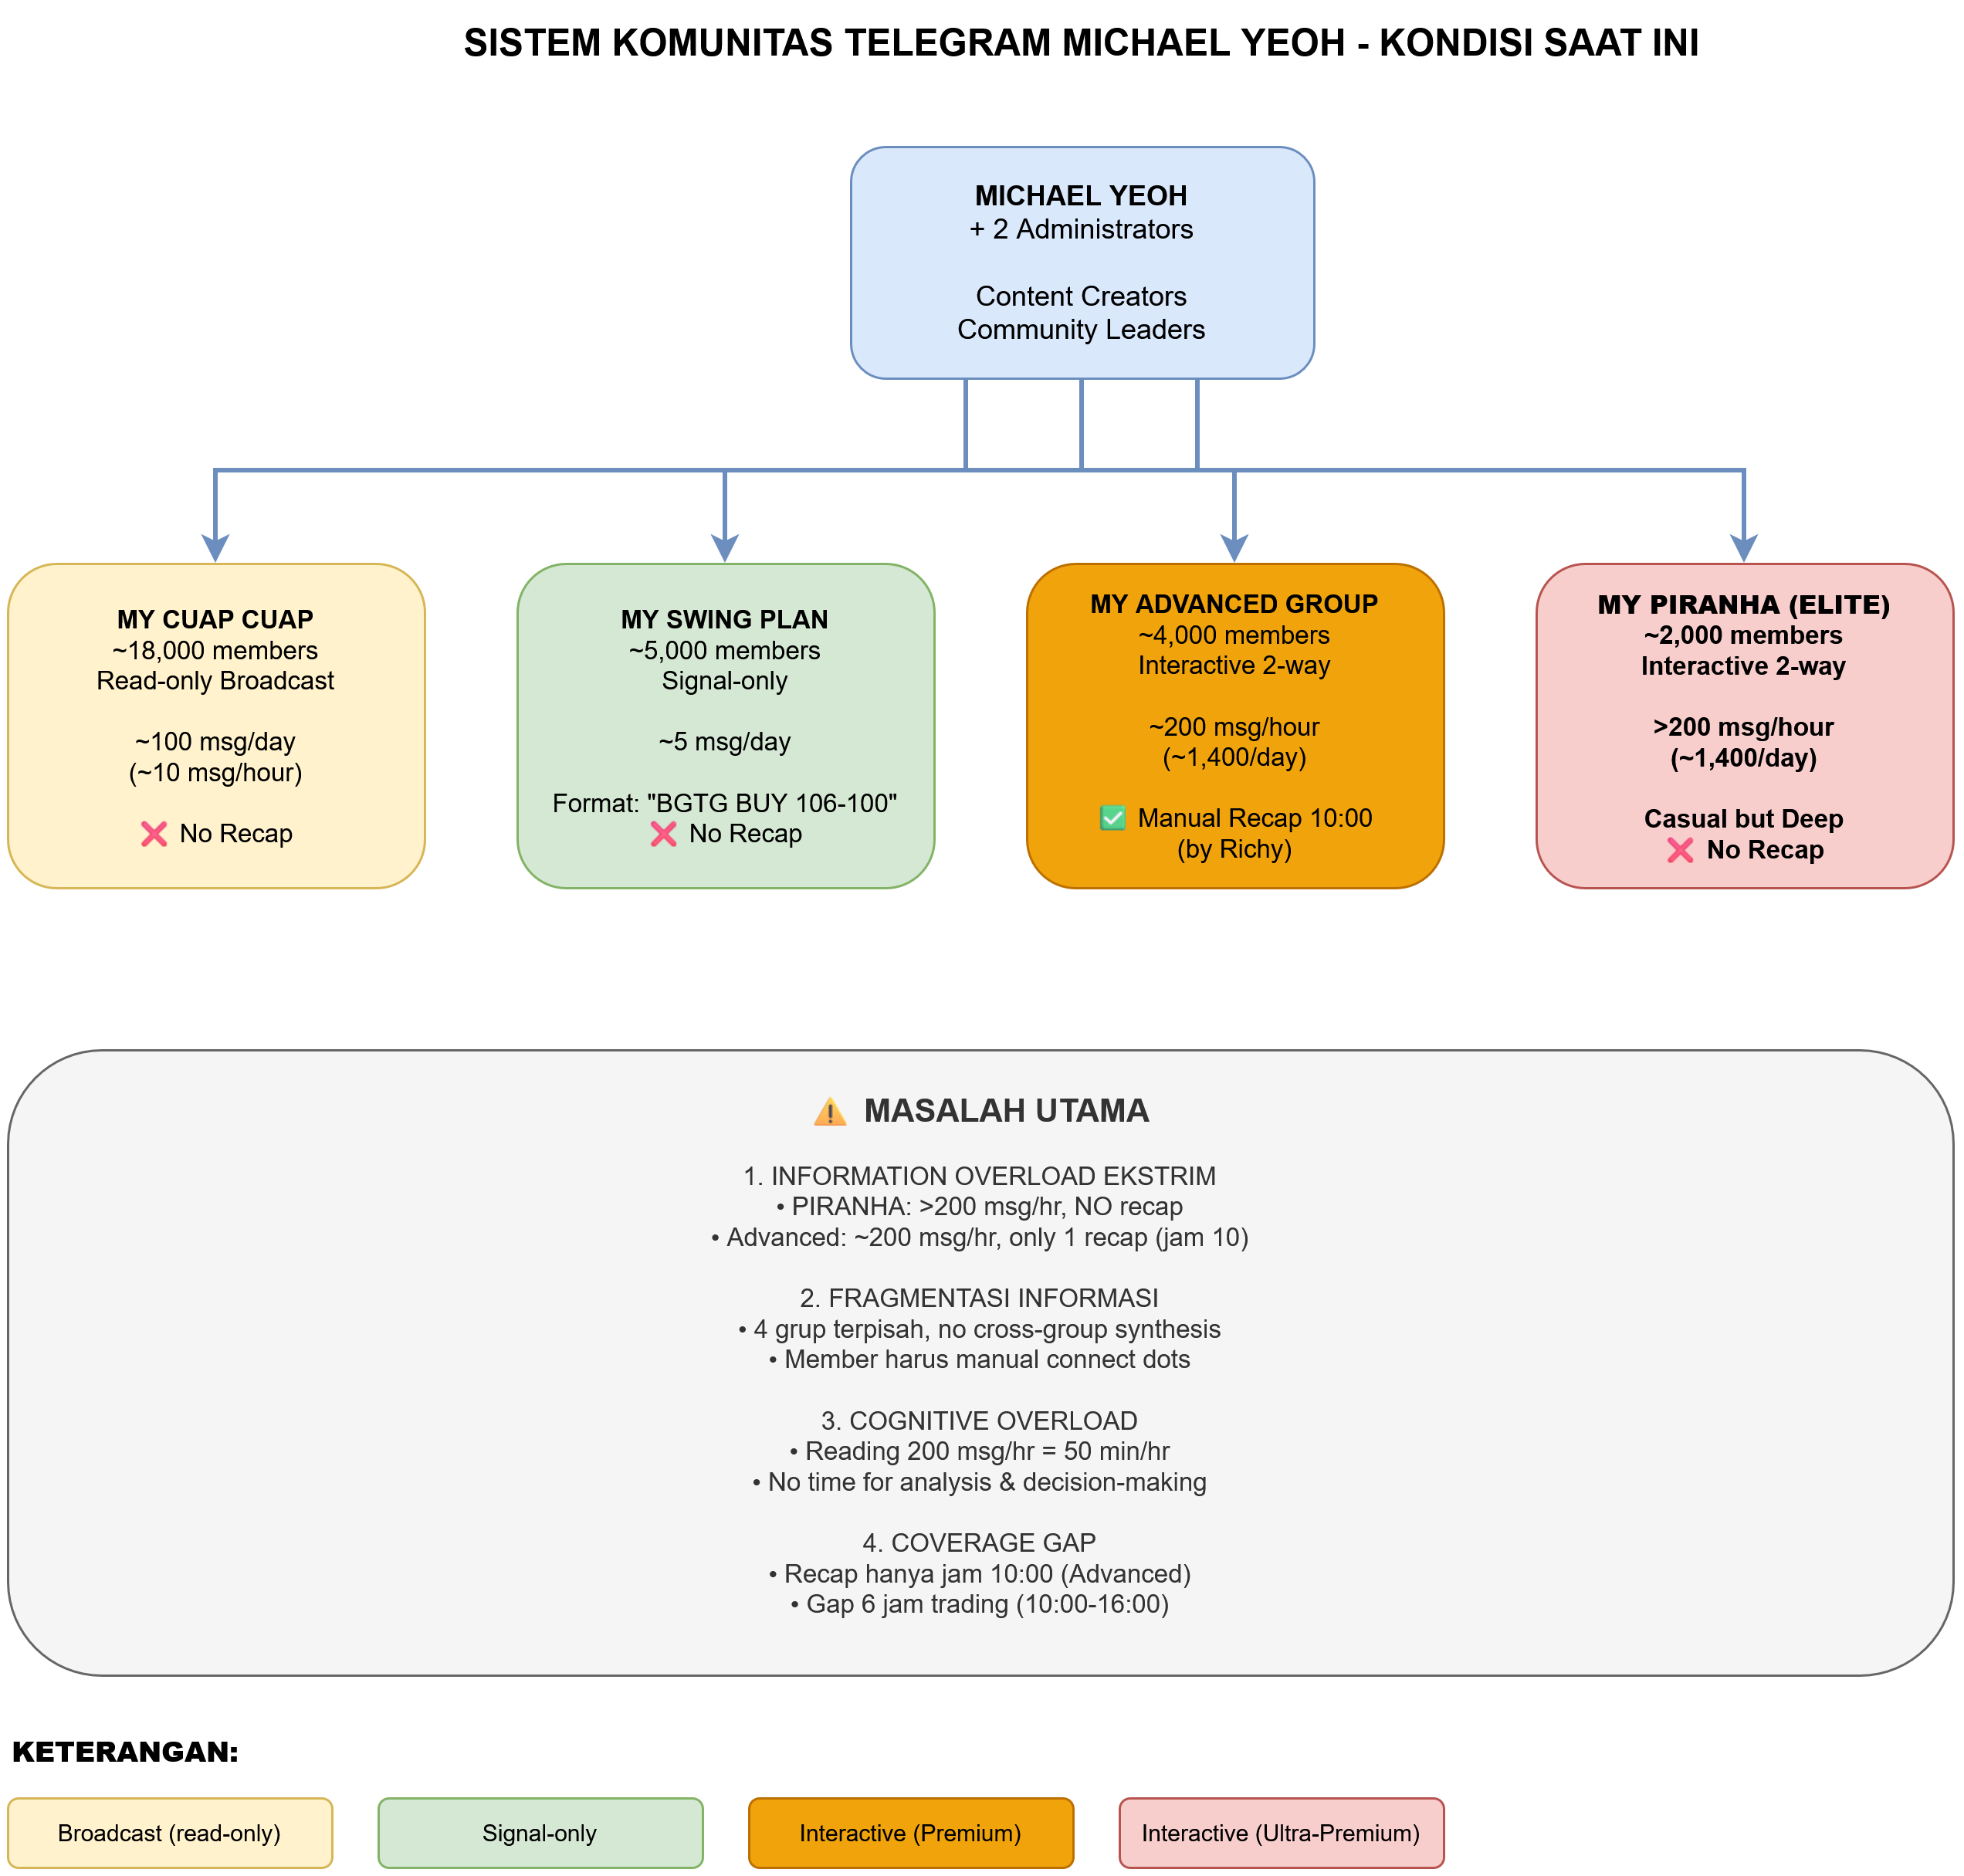
\includegraphics[width=0.9\textwidth]{image/current-state-diagram.png}
  \caption{Model konseptual sistem komunikasi komunitas Telegram Michael Yeoh saat ini}
  \label{fig:current-system}
\end{figure}

Struktur hierarkis komunitas terdiri dari empat grup dengan karakteristik berbeda yang dapat dilihat pada Tabel \ref{tab:group-characteristics}. Setiap grup memiliki fungsi spesifik dalam ekosistem informasi komunitas, dengan kompleksitas komunikasi yang meningkat seiring level hierarki.

\begin{table}[H]
\centering
\caption{Karakteristik grup dalam komunitas Telegram Michael Yeoh}
\label{tab:group-characteristics}
\begin{tabular}{|p{3cm}|p{2.5cm}|p{2.5cm}|p{3cm}|p{2.5cm}|}
\hline
\textbf{Aspek} & \textbf{Cuap Cuap} & \textbf{Swing Plan} & \textbf{Advanced} & \textbf{PIRANHA} \\
\hline
Jumlah Member & ~18.000 & ~5.000 & ~4.000 & ~2.000 \\
\hline
Tipe Komunikasi & Broadcast (\textit{read-only}) & Signal-only & Interaktif 2-arah & Interaktif 2-arah \\
\hline
Volume Pesan & ~100 msg/hari (~10/jam) & ~5 msg/hari & ~200 msg/jam & >200 msg/jam \\
\hline
Konten Utama & Edukasi umum, berita pasar & Sinyal beli/jual terstruktur & Diskusi analisis teknikal & Debat strategi expert \\
\hline
\textit{Recap} Manual & Tidak ada & Tidak ada & 1× per hari (jam 10:00) & Tidak ada \\
\hline
Tingkat Masalah & Rendah & Minimal & Tinggi & Sangat Tinggi \\
\hline
\end{tabular}
\end{table}

Setiap grup dalam hierarki komunitas memiliki peran dan dinamika komunikasi yang berbeda. Grup MY Cuap Cuap berfungsi sebagai kanal informasi umum dengan mode \textit{read-only}, di mana hanya administrator dan Michael Yeoh yang dapat mengirim pesan. Konten utama meliputi edukasi pasar saham, analisis makroekonomi, dan pengumuman penting. Dengan volume sekitar 100 pesan per hari atau rata-rata 10 pesan per jam, grup ini memiliki tingkat \textit{information overload} yang relatif rendah.

Grup MY Swing Plan merupakan kanal khusus untuk distribusi sinyal \textit{trading} dengan format terstruktur seperti "BGTG BUY 106-100 SL 98 porsi 5\%". Volume pesan sangat rendah (~5 pesan per hari) karena sifatnya yang spesifik dan terarah. Grup ini tidak mengalami masalah \textit{information overload}, namun menjadi bagian penting dari ekosistem informasi yang perlu disintesis dengan diskusi di grup lain untuk memberikan konteks komprehensif.

Grup MY Advanced Group adalah grup premium pertama dengan komunikasi interaktif dua arah, di mana sekitar 4.000 anggota dapat berdiskusi secara langsung. Volume pesan mencapai sekitar 200 pesan per jam selama jam perdagangan aktif (09:00-16:00), menghasilkan total sekitar 1.400 pesan per hari. Grup ini memiliki satu rangkuman manual yang dibuat oleh asisten bernama Richy Matthew Ashari setiap hari pada jam 10:00 pagi. Rangkuman manual ini mencakup kondisi pasar dan pergerakan saham-saham prioritas (\textit{PP stocks}) dengan format yang mencantumkan level support, resistance, dan analisis kekuatan saham. Namun, rangkuman ini hanya mencakup satu jam pertama perdagangan (09:00-10:00), meninggalkan gap informasi selama enam jam perdagangan berikutnya (10:00-16:00).

Grup MY PIRANHA merupakan grup ultra-premium dengan 2.000 anggota elite dan mengalami volume pesan tertinggi, melebihi 200 pesan per jam, menghasilkan lebih dari 1.400 pesan per hari. Berbeda dengan Advanced Group, PIRANHA tidak memiliki rangkuman manual sama sekali. Diskusi di grup ini cenderung lebih kasual dalam gaya komunikasi namun sangat mendalam secara konten, dengan debat strategi investasi antar investor berpengalaman. Paradoks "kasual namun \textit{high-volume}" ini menciptakan tantangan ekstraksi sinyal yang unik, karena informasi penting sering tersembunyi dalam percakapan informal yang memerlukan pemahaman konteks mendalam.

Aliran informasi dalam ekosistem komunitas bersifat hierarkis dan fragmentasi. Michael Yeoh dan dua administrator lainnya dapat memposting di semua grup, menciptakan aliran informasi vertikal dari puncak hierarki. Namun, anggota di level berbeda tidak dapat mengakses informasi di grup yang lebih tinggi kecuali mereka menjadi anggota grup tersebut. Hal ini menciptakan fragmentasi informasi di mana analisis makro di Cuap Cuap, sinyal konkret di Swing Plan, diskusi implementasi di Advanced, dan debat strategi di PIRANHA terpisah satu sama lain. Anggota yang merupakan bagian dari multiple grup harus secara manual melakukan sintesis informasi lintas grup, yang memerlukan waktu dan kemampuan analisis yang signifikan.

\subsection{Identifikasi Masalah Sistem Saat Ini}

Berdasarkan analisis terhadap model konseptual sistem saat ini, terdapat tiga kategori masalah utama yang menjadi fokus penelitian ini: \textit{information overload} dengan intensitas ekstrim di grup premium, fragmentasi informasi lintas struktur hierarkis, dan keterbatasan kognitif anggota dalam memproses volume informasi tinggi.

\subsubsection{\textit{Information Overload} Ekstrim di Grup PIRANHA}

Grup PIRANHA mengalami tingkat \textit{information overload} paling parah dalam ekosistem komunitas. Dengan volume melebihi 200 pesan per jam selama jam perdagangan (09:00-16:00), grup ini menghasilkan lebih dari 1.400 pesan per hari. Tidak adanya mekanisme rangkuman otomatis atau manual membuat anggota dihadapkan pada dua pilihan yang sama-sama suboptimal: (1) memantau diskusi secara \textit{real-time} yang memerlukan perhatian konstan selama tujuh jam perdagangan, atau (2) melakukan \textit{catch-up} dengan membaca ratusan pesan secara retrospektif, yang berisiko kehilangan konteks temporal dan relevansi diskusi.

Karakteristik unik dari diskusi PIRANHA yang kasual namun mendalam memperburuk masalah ini. Tidak seperti diskusi terstruktur di grup lain, informasi kritis di PIRANHA sering tersembunyi dalam percakapan informal tanpa penanda eksplisit seperti format sinyal trading atau header topik. Ekstraksi sinyal dari diskusi kasual memerlukan pemahaman konteks yang dalam, yang sulit dilakukan ketika anggota harus memproses volume pesan yang sangat tinggi dalam waktu terbatas.

Dampak kuantitatif dari masalah ini dapat diestimasi menggunakan kerangka \textit{Cognitive Load Theory}. Jika diasumsikan rata-rata waktu baca dan pemahaman per pesan adalah 15 detik, maka untuk membaca 200 pesan memerlukan 50 menit, mendekati satu jam penuh. Selama jam perdagangan yang berlangsung selama tujuh jam, anggota yang mencoba membaca semua pesan akan menghabiskan hampir seluruh waktu mereka hanya untuk konsumsi informasi, tanpa waktu untuk analisis dan pengambilan keputusan. Situasi ini jelas tidak sustainable dan bertentangan dengan tujuan komunitas untuk memfasilitasi pengambilan keputusan investasi yang efektif.

\subsubsection{\textit{Information Overload} Tinggi di Grup Advanced dengan \textit{Coverage Gap}}

Grup Advanced Group, meskipun memiliki satu rangkuman manual harian, masih mengalami masalah \textit{information overload} yang signifikan dengan beberapa dimensi. Pertama, volume pesan sekitar 200 pesan per jam menghasilkan total sekitar 1.400 pesan per hari, angka yang hampir identik dengan PIRANHA. Kedua, rangkuman manual yang ada hanya mencakup satu jam pertama perdagangan (09:00-10:00), meninggalkan gap informasi selama enam jam berikutnya.

Gap \textit{coverage} temporal ini menciptakan masalah asimetri informasi. Anggota yang dapat memantau diskusi pada pagi hari memiliki akses ke rangkuman manual jam 10:00 yang menyediakan konteks diskusi pagi. Namun, anggota yang bergabung setelah jam 10:00 atau yang tidak dapat memantau diskusi siang hingga sore hari (10:00-16:00) kehilangan konteks penting dari diskusi di periode tersebut. Mengingat bahwa kondisi pasar dan sentimen dapat berubah drastis dalam beberapa jam, gap ini dapat menyebabkan pengambilan keputusan berdasarkan informasi yang tidak lengkap atau \textit{outdated}.

Keterbatasan rangkuman manual juga terletak pada skalabilitas dan konsistensi. Pembuatan rangkuman bergantung pada satu individu (Richy Matthew Ashari) dengan ketersediaan waktu dan perspektif subjektif tertentu. Model ini tidak dapat di-\textit{scale} untuk memberikan \textit{coverage} yang lebih komprehensif sepanjang hari tanpa menambah jumlah personel secara signifikan, yang tidak efisien dari segi biaya dan koordinasi. Lebih lanjut, tidak ada jaminan konsistensi format dan kedalaman analisis antar rangkuman karena sifatnya yang manual.

\subsubsection{Fragmentasi Informasi Lintas Struktur Hierarkis}

Struktur hierarkis empat tingkat komunitas, meskipun dirancang untuk menyediakan nilai berbeda di setiap level, menciptakan masalah fragmentasi informasi yang sistemik. Informasi yang relevan untuk pengambilan keputusan investasi tersebar di empat grup dengan sedikit mekanisme sintesis eksplisit. Sebagai contoh, skenario tipikal dapat melibatkan: (1) Michael Yeoh memposting analisis makroekonomi tentang kondisi likuiditas pasar di grup Cuap Cuap, (2) sinyal konkret untuk beberapa saham diberikan di Swing Plan berdasarkan analisis tersebut, (3) diskusi tentang implementasi strategi dan manajemen risiko berlangsung di Advanced Group, dan (4) debat mendalam tentang potensi \textit{upside} versus \textit{downside} terjadi di PIRANHA.

Untuk mendapatkan pemahaman komprehensif, seorang anggota yang merupakan bagian dari semua grup harus secara manual: (1) membaca dan memahami konten di keempat grup, (2) mengidentifikasi hubungan semantik antar informasi, (3) mensintesis informasi menjadi \textit{actionable insight}, dan (4) melakukan ini secara berulang sepanjang hari karena informasi terus mengalir. Proses ini memerlukan \textit{cognitive switching cost} yang tinggi karena anggota harus berpindah antar konteks komunikasi yang berbeda (broadcast vs interaktif, formal vs kasual, umum vs spesifik).

Masalah ini diperparah oleh fakta bahwa sebagian besar anggota tidak memiliki akses ke semua grup. Anggota di Cuap Cuap dan Swing Plan tidak dapat mengakses diskusi mendalam di Advanced atau PIRANHA, menciptakan asimetri informasi struktural. Sementara itu, anggota premium yang memiliki akses ke multiple grup menghadapi beban kognitif yang berlebihan untuk melakukan sintesis manual. Tidak ada mekanisme dalam sistem saat ini yang secara otomatis mengagregasi dan mensintesis informasi lintas grup untuk memberikan pandangan holistik.

\subsubsection{Keterbatasan Kapasitas Kognitif dan Dampaknya terhadap Kualitas Keputusan}

Berdasarkan kerangka \textit{Cognitive Load Theory} yang telah dibahas dalam Bab \ref{chap:studi-literatur}, kapasitas memori kerja manusia memiliki keterbatasan fundamental dalam memproses informasi secara simultan. Dalam konteks komunitas Telegram finansial dengan volume pesan yang sangat tinggi, anggota menghadapi beban kognitif yang melampaui kapasitas optimal pada beberapa dimensi.

Pertama, \textit{intrinsic cognitive load} yang tinggi inheren dalam domain finansial itu sendiri. Analisis investasi saham memerlukan pemahaman tentang analisis teknikal, fundamental, sentimen pasar, manajemen risiko, dan psikologi \textit{trading}. Kompleksitas intrinsik ini tidak dapat dikurangi karena merupakan bagian esensial dari domain.

Kedua, \textit{extraneous cognitive load} yang ditambahkan oleh desain sistem saat ini sangat signifikan. Antarmuka Telegram dengan notifikasi konstan, fragmentasi informasi antar grup, kurangnya struktur hierarkis dalam penyajian pesan, dan tidak adanya mekanisme filter atau prioritas menciptakan beban kognitif tambahan yang tidak berkontribusi langsung pada pembelajaran atau pengambilan keputusan. Desain sistem yang mengharuskan anggota untuk scroll ratusan pesan, membedakan informasi penting dari \textit{noise}, dan melakukan sintesis manual meningkatkan \textit{extraneous load} secara dramatis.

Ketiga, kapasitas untuk \textit{germane cognitive load} yang berkontribusi pada pemahaman mendalam dan pembentukan skema mental investasi yang baik menjadi terbatas. Ketika sebagian besar sumber daya kognitif digunakan untuk mengatasi beban informasi (\textit{intrinsic} dan \textit{extraneous}), kapasitas untuk refleksi, analisis mendalam, dan integrasi pengetahuan baru menjadi terbatas.

Dampak dari situasi ini terhadap kualitas pengambilan keputusan dapat bermanifestasi dalam beberapa cara. Anggota mungkin mengalami \textit{decision fatigue}, di mana kualitas keputusan menurun seiring waktu karena deplesi sumber daya kognitif. Alternatifnya, anggota mungkin mengembangkan strategi \textit{satisficing}, di mana mereka membuat keputusan berdasarkan subset informasi yang mudah diakses daripada melakukan analisis komprehensif. Dalam kasus terburuk, anggota mungkin mengalami \textit{analysis paralysis}, di mana volume informasi yang berlebihan menyebabkan ketidakmampuan untuk membuat keputusan sama sekali.

Penelitian empiris yang akan dilakukan dalam tugas akhir ini bertujuan untuk mengukur dampak dari masalah-masalah ini dan mengevaluasi sejauh mana sistem rangkuman otomatis dapat mereduksi beban kognitif dan meningkatkan efektivitas pengambilan keputusan anggota komunitas.

% ==========================================
\section{Analisis Kebutuhan}
\label{sec:analisis-kebutuhan}

Berdasarkan identifikasi masalah pada sistem saat ini, bagian ini menganalisis kebutuhan sistem rangkuman otomatis dari perspektif \textit{stakeholder} yang berbeda, serta mendefinisikan kebutuhan fungsional dan non-fungsional yang harus dipenuhi oleh solusi yang diusulkan.

\subsection{Identifikasi \textit{Stakeholder} dan \textit{Pain Points}}

Sistem rangkuman otomatis yang diusulkan melayani beberapa kelompok \textit{stakeholder} dengan \textit{pain points} dan kebutuhan yang berbeda. Pemahaman mendalam terhadap kebutuhan setiap \textit{stakeholder} penting untuk desain sistem yang efektif dan \textit{user-centric}.

\subsubsection{Anggota Grup PIRANHA (Target Primer)}

Anggota grup PIRANHA, yang berjumlah sekitar 2.000 investor ultra-premium, merupakan \textit{stakeholder} primer dengan \textit{pain points} paling akut. \textit{Pain point} utama adalah \textit{information overload} ekstrim dengan volume lebih dari 200 pesan per jam yang tidak memiliki mekanisme rangkuman sama sekali. Saat ini, mereka mengandalkan \textit{workaround} manual seperti scrolling periodik atau pencarian pengguna spesifik yang dipercaya, namun pendekatan ini memiliki keterbatasan signifikan dalam hal efisiensi waktu dan risiko kehilangan informasi penting.

Kebutuhan spesifik kelompok ini meliputi: (1) rangkuman periodik yang dapat memberikan snapshot diskusi tanpa harus membaca ratusan pesan, (2) identifikasi topik dan saham yang paling banyak dibahas untuk prioritisasi perhatian, (3) ekstraksi sinyal dari percakapan kasual yang informal namun substantif, dan (4) diferensiasi kontribusi dari investor berpengalaman versus diskusi umum. Mengingat karakteristik anggota PIRANHA sebagai investor berpengalaman dengan \textit{time value} yang tinggi, efisiensi waktu akses informasi menjadi nilai proposition utama.

\subsubsection{Anggota Grup Advanced (Target Sekunder)}

Anggota grup Advanced, dengan sekitar 4.000 anggota premium, menghadapi \textit{pain points} yang serupa namun dengan nuansa berbeda. Meskipun mereka memiliki akses ke rangkuman manual jam 10:00, terdapat gap \textit{coverage} signifikan untuk perdagangan siang hingga sore (10:00-16:00). \textit{Workaround} saat ini adalah memeriksa grup secara periodik, namun ini mengganggu produktivitas dan fokus pada aktivitas lain.

Kebutuhan kelompok ini meliputi: (1) rangkuman tambahan sepanjang hari untuk melengkapi rangkuman manual eksisting, (2) informasi tentang perubahan sentimen atau topik baru yang muncul setelah jam 10:00, dan (3) sintesis lintas grup yang menghubungkan informasi dari Cuap Cuap dan Swing Plan dengan diskusi di Advanced. Kelompok ini juga akan mendapat manfaat dari standardisasi format rangkuman yang konsisten, mengingat variabilitas dalam rangkuman manual.

\subsubsection{Anggota Cuap Cuap dan Swing Plan}

Anggota grup Cuap Cuap (~18.000) dan Swing Plan (~5.000) menghadapi \textit{pain points} yang berbeda, yaitu keterbatasan akses ke diskusi mendalam yang terjadi di grup premium. Meskipun mereka tidak mengalami \textit{information overload} di grup mereka sendiri, mereka kehilangan konteks penting tentang bagaimana analisis umum atau sinyal trading diimplementasikan dan didiskusikan oleh komunitas premium.

Kebutuhan kelompok ini meliputi: (1) akses (meskipun mungkin terbatas) ke insight dari diskusi premium tanpa harus upgrade keanggotaan, (2) pemahaman tentang sentimen komunitas secara keseluruhan terhadap saham atau kondisi pasar tertentu, dan (3) validasi bahwa sinyal yang mereka terima memiliki dukungan diskusi substantif di tingkat yang lebih tinggi. Sistem rangkuman dapat menyediakan nilai ini sambil tetap menghormati struktur premium komunitas.

\subsubsection{Michael Yeoh dan Tim Administrator}

Michael Yeoh dan dua administrator lainnya memiliki perspektif yang berbeda sebagai \textit{content creator} dan pengelola komunitas. \textit{Pain point} utama mereka adalah kesulitan memastikan bahwa informasi penting yang mereka distribusikan benar-benar sampai dan dipahami oleh semua anggota yang relevan. Keterbatasan rangkuman manual adalah bahwa hanya satu orang (Richy) yang dapat mengalokasikan waktu untuk ini, dan tidak \textit{scalable} untuk memberikan \textit{coverage} yang lebih komprehensif.

Kebutuhan kelompok ini meliputi: (1) alat untuk broadcast insight teragregasi yang dapat menjangkau lebih banyak anggota secara efektif, (2) pemahaman tentang topik dan sentimen yang dominan dalam komunitas untuk informed \textit{content strategy}, (3) reduksi beban manual dalam pembuatan rangkuman, dan (4) mekanisme untuk memastikan konsistensi kualitas rangkuman terlepas dari ketersediaan personel.

\subsection{Kebutuhan Fungsional}

Berdasarkan analisis \textit{stakeholder} dan masalah sistem saat ini, Tabel \ref{tab:functional-requirements} merangkum kebutuhan fungsional sistem rangkuman otomatis yang diusulkan. Kebutuhan ini dikategorikan berdasarkan prioritas menggunakan metode MoSCoW (\textit{Must have}, \textit{Should have}, \textit{Could have}, \textit{Won't have}).

\begin{longtable}{|p{1.5cm}|p{8cm}|p{2cm}|p{3cm}|}
\caption{Kebutuhan fungsional sistem rangkuman otomatis} 
\label{tab:functional-requirements} \\
\hline
\textbf{ID} & \textbf{Kebutuhan Fungsional} & \textbf{Prioritas} & \textbf{Keterangan} \\
\hline
\endfirsthead

\multicolumn{4}{c}%
{{\tablename\ \thetable{} -- lanjutan dari halaman sebelumnya}} \\
\hline
\textbf{ID} & \textbf{Kebutuhan Fungsional} & \textbf{Prioritas} & \textbf{Keterangan} \\
\hline
\endhead

\hline \multicolumn{4}{r}{{Lanjut ke halaman berikutnya}} \\
\endfoot

\hline
\endlastfoot

FR-01 & Sistem harus dapat mengumpulkan pesan dari empat grup Telegram (MY Cuap Cuap, MY Swing Plan, MY Advanced Group, MY PIRANHA) secara \textit{real-time} & MUST & Fondasi sistem untuk akuisisi data \\
\hline

FR-02 & Sistem harus dapat mengekstrak entitas finansial (nama perusahaan, kode ticker saham) menggunakan model \textit{cahya/bert-base-indonesian-NER} dan \textit{whitelist} ticker dari \textit{Indonesia Stock Exchange} & MUST & Identifikasi aset yang dibahas \\
\hline

FR-03 & Sistem harus dapat menganalisis emosi pesan menggunakan \textit{indonesian-roberta-base-emotion-classifier} untuk mendeteksi spektrum emosi (ketakutan, kegembiraan, kemarahan) & MUST & Analisis sentimen psikologis pasar \\
\hline

FR-04 & Sistem harus dapat mengidentifikasi topik diskusi dominan dalam setiap periode waktu menggunakan BERTopic & MUST & Pemodelan topik untuk kategorisasi \\
\hline

FR-05 & Sistem harus menerapkan \textit{weighted influence system} dengan bobot: Michael Yeoh (4×), Administrator (3×), VIP members (2×), Regular members (1×) & MUST & Filter intelijen berbasis hierarki \\
\hline

FR-06 & Sistem harus menghasilkan rangkuman secara otomatis pada interval waktu tetap (11:00, 12:00, 14:00, 15:00, 16:00) & MUST & Otomasi periodik \\
\hline

FR-07 & Rangkuman harus merupakan sintesis lintas-grup (\textit{cross-group merged}) yang mengintegrasikan informasi dari keempat grup dalam satu dokumen koheren & MUST & Sintesis holistik \\
\hline

FR-08 & Format rangkuman harus \textit{mixed} yang menggabungkan bullet points untuk informasi terstruktur dan paragraf naratif untuk konteks & MUST & Readability dan comprehensiveness \\
\hline

FR-09 & Sistem TIDAK boleh memproses pesan yang telah di-\textit{unsend} oleh pengirim untuk menghormati privasi & MUST & Perlindungan privasi eksplisit \\
\hline

FR-10 & Sistem harus mengirim rangkuman yang dihasilkan ke kanal Telegram output yang dedicated melalui Telegram Bot API & MUST & Distribusi otomatis \\
\hline

FR-11 & Sistem harus menyimpan rangkuman historis beserta metadata (timestamp, jumlah pesan diproses, topik terdeteksi) dalam basis data & SHOULD & Persistensi data dan audit trail \\
\hline

FR-12 & Sistem harus mendukung query untuk mengakses rangkuman periode tertentu (harian, mingguan) melalui perintah bot & COULD & Akses retroaktif \\
\hline
\end{longtable}

\subsection{Kebutuhan Non-Fungsional}

Kebutuhan non-fungsional mendefinisikan atribut kualitas sistem yang harus dipenuhi untuk memastikan sistem dapat beroperasi secara efektif dalam konteks \textit{real-world} komunitas Telegram finansial. Tabel \ref{tab:nonfunctional-requirements} merangkum kebutuhan non-fungsional beserta target metrik yang dapat diukur.

\begin{longtable}{|p{1.5cm}|p{3.5cm}|p{3.5cm}|p{5cm}|}
\caption{Kebutuhan non-fungsional sistem rangkuman otomatis} 
\label{tab:nonfunctional-requirements} \\
\hline
\textbf{ID} & \textbf{Aspek} & \textbf{Target Metrik} & \textbf{Keterangan} \\
\hline
\endfirsthead

\multicolumn{4}{c}%
{{\tablename\ \thetable{} -- lanjutan dari halaman sebelumnya}} \\
\hline
\textbf{ID} & \textbf{Aspek} & \textbf{Target Metrik} & \textbf{Keterangan} \\
\hline
\endhead

\hline \multicolumn{4}{r}{{Lanjut ke halaman berikutnya}} \\
\endfoot

\hline
\endlastfoot

NFR-01 & \textit{Response Time} & Rangkuman harus selesai dihasilkan dalam waktu kurang dari 5 menit setelah akhir periode pengumpulan & Relevansi temporal untuk grup PIRANHA yang sangat aktif \\
\hline

NFR-02 & Akurasi NER & \textit{Precision} dan \textit{Recall} deteksi ticker saham Indonesia harus mencapai minimal 80\% & Kualitas ekstraksi entitas finansial \\
\hline

NFR-03 & Kualitas \textit{Topic Modeling} & \textit{Coherence score} BERTopic harus mencapai minimal 0.5 & Topik yang dihasilkan harus interpretatif dan bermakna \\
\hline

NFR-04 & \textit{System Uptime} & Ketersediaan sistem harus mencapai minimal 95\% selama jam perdagangan (09:00-16:00) & Reliabilitas operasional \\
\hline

NFR-05 & \textit{Scalability} & Sistem harus mampu menangani lebih dari 250 pesan per jam per grup tanpa degradasi performa & \textit{Future-proof} untuk pertumbuhan komunitas \\
\hline

NFR-06 & Privasi & Zero kebocoran data; pesan yang di-\textit{unsend} harus dikecualikan dari pemrosesan & Kepatuhan terhadap prinsip privasi \\
\hline

NFR-07 & \textit{Usability} & Rangkuman harus dapat dibaca dan dipahami dalam waktu kurang dari 3 menit oleh anggota rata-rata & Target \textit{user experience} \\
\hline

NFR-08 & Lokalisasi & Semua output rangkuman harus dalam Bahasa Indonesia dengan terminologi finansial yang sesuai & Aksesibilitas untuk komunitas lokal \\
\hline

NFR-09 & Efisiensi Biaya & Biaya operasional Groq API untuk inferensi LLM harus kurang dari \$50 per bulan untuk 18 rangkuman per hari & Keberlanjutan finansial \\
\hline
\end{longtable}

Target metrik pada kebutuhan non-fungsional ini akan menjadi dasar untuk evaluasi sistem pada fase \textit{Evaluation} metodologi DSRM. Beberapa metrik seperti akurasi NER dan kualitas topic modeling dapat diukur secara objektif melalui evaluasi teknis. Metrik lain seperti \textit{usability} dan efisiensi waktu akses akan diukur melalui survei \textit{feedback} pengguna yang akan dilakukan selama fase pengujian sistem.

% ==========================================
\section{Analisis Alternatif Solusi}
\label{sec:alternatif-solusi}

Untuk mengatasi masalah \textit{information overload} dan fragmentasi informasi yang telah diidentifikasi, terdapat beberapa pendekatan alternatif yang dapat dipertimbangkan. Bagian ini menganalisis empat alternatif utama beserta kelebihan dan kekurangan masing-masing, diikuti dengan analisis pemilihan solusi menggunakan \textit{decision matrix}.

\subsection{Alternatif Pendekatan untuk Mereduksi \textit{Information Overload}}

\subsubsection{Alternatif 1: Ekspansi \textit{Manual Curation} (Status Quo yang Ditingkatkan)}

Alternatif pertama adalah mempertahankan pendekatan rangkuman manual namun dengan ekspansi signifikan dalam frekuensi dan \textit{coverage}. Pendekatan ini melibatkan perekrutan dua hingga tiga asisten tambahan untuk membuat rangkuman multiple kali per hari di semua grup, termasuk PIRANHA yang saat ini tidak memiliki rangkuman manual.

\textbf{Kelebihan:}
\begin{itemize}
\item Kualitas penilaian manusia yang superior dalam memahami nuansa konteks dan relevansi informasi
\item Tidak ada risiko teknis atau ketergantungan pada sistem \textit{machine learning} yang mungkin menghasilkan output yang tidak akurat
\item Fleksibilitas dalam menyesuaikan gaya dan format rangkuman berdasarkan feedback komunitas secara \textit{ad-hoc}
\end{itemize}

\textbf{Kekurangan:}
\begin{itemize}
\item Biaya operasional tinggi: dengan asumsi kompensasi Rp 5 juta per bulan per asisten, total biaya untuk tiga asisten adalah Rp 15 juta per bulan, atau Rp 180 juta per tahun
\item Masalah skalabilitas fundamental: untuk memberikan \textit{coverage} enam kali per hari di empat grup memerlukan 24 instansi rangkuman manual per hari, yang sulit dikoordinasikan dan memastikan konsistensi
\item Bias subjektif dan variabilitas antar-\textit{curator}: setiap asisten mungkin memiliki perspektif dan prioritas berbeda dalam memilih informasi yang dianggap penting
\item \textit{Human fatigue} dan potensi kesalahan: membuat rangkuman berkualitas tinggi secara konsisten memerlukan fokus dan energi kognitif yang tinggi, yang sulit dipertahankan dalam jangka panjang
\item Ketidakmampuan untuk menerapkan \textit{weighted influence} secara algoritmik dan konsisten
\end{itemize}

\subsubsection{Alternatif 2: Bot Filter Berbasis Aturan (\textit{Rule-Based Keyword Bot})}

Alternatif kedua adalah mengembangkan bot Telegram sederhana yang memfilter pesan berdasarkan aturan \textit{keyword} dan pola teks yang telah ditentukan sebelumnya. Bot akan mendeteksi kata kunci seperti nama saham (PTRO, BBCA, GOTO), kata-kata sinyal (\textit{buy}, \textit{sell}, \textit{resistance}, \textit{support}), dan mengirimkan pesan yang cocok ke kanal output.

\textbf{Kelebihan:}
\begin{itemize}
\item Implementasi cepat dan mudah: sistem berbasis aturan dapat dibangun dalam 1-2 minggu
\item Biaya operasional sangat rendah: hosting bot sederhana dapat dilakukan dengan biaya kurang dari \$5 per bulan
\item Transparan dan dapat diprediksi: aturan filter jelas dan dapat disesuaikan oleh administrator tanpa keahlian \textit{machine learning}
\end{itemize}

\textbf{Kekurangan:}
\begin{itemize}
\item Tidak ada pemahaman konteks: sistem \textit{keyword matching} tidak dapat membedakan antara diskusi substantif tentang saham versus sekadar menyebut nama saham secara kasual
\item \textit{False positive} tinggi: banyak pesan yang mengandung keyword tetapi tidak informatif akan difilter
\item \textit{False negative} tinggi: informasi penting yang tidak menggunakan keyword eksplisit akan terlewat
\item Tidak dapat melakukan sintesis atau agregasi: bot hanya meneruskan pesan individual tanpa menciptakan rangkuman yang koheren
\item \textit{Brittle} dan memerlukan pemeliharaan konstan: setiap perubahan dalam cara komunitas berkomunikasi memerlukan update manual aturan
\item Tidak dapat menerapkan \textit{weighted influence} atau analisis sentimen yang kompleks
\end{itemize}

\subsubsection{Alternatif 3: Bot Rangkuman Berbasis \textit{AI} dengan NLP Khusus Domain (DIUSULKAN)}

Alternatif ketiga, yang merupakan solusi yang diusulkan dalam penelitian ini, adalah mengembangkan sistem rangkuman otomatis berbasis \textit{artificial intelligence} dengan \textit{pipeline} NLP yang dioptimalkan untuk domain finansial Indonesia. Sistem ini mengintegrasikan multiple komponen: ekstraksi entitas menggunakan \textit{bert-based-indonesian-NER}, analisis emosi dengan \textit{indonesian-roberta-base-emotion-classifier}, pemodelan topik dengan BERTopic, \textit{weighted influence algorithm}, dan generasi rangkuman dengan \textit{large language model} (Llama 3.1 70B via Groq API).

\textbf{Kelebihan:}
\begin{itemize}
\item Pemahaman konteks berbasis semantik: model NLP dapat memahami makna pesan di luar sekadar \textit{keyword matching}
\item Skalabilitas tinggi: setelah dibangun, sistem dapat memproses empat grup dengan enam rangkuman per hari (total 24 rangkuman) tanpa penambahan biaya proporsional
\item \textit{Weighted influence system} algoritmik: dapat secara konsisten menerapkan bobot berbeda berdasarkan peran pengirim (Michael Yeoh 4×, admin 3×, VIP 2×, regular 1×) yang sulit dilakukan secara manual
\item Optimisasi untuk domain finansial Indonesia: penggunaan model yang di-\textit{fine-tune} untuk bahasa Indonesia dan entitas finansial lokal (kode ticker BEI, nama perusahaan Indonesia)
\item Sintesis lintas-grup otomatis: kemampuan untuk mengintegrasikan informasi dari empat grup dalam satu rangkuman koheren
\item Perlindungan privasi built-in: mekanisme untuk mengecualikan pesan yang di-\textit{unsend}
\item Biaya operasional terjangkau: estimasi \$30-50 per bulan untuk Groq API, jauh lebih rendah dibanding Rp 15 juta per bulan untuk solusi manual
\item Konsistensi output: format dan kualitas rangkuman stabil karena dihasilkan oleh sistem yang sama
\end{itemize}

\textbf{Kekurangan:}
\begin{itemize}
\item Kompleksitas teknis tinggi: memerlukan keahlian dalam NLP, \textit{machine learning}, dan integrasi sistem
\item Ketergantungan pada kualitas model: akurasi sistem terbatas pada performa model NER (target 80\%), topic modeling, dan LLM
\item \textit{Vendor lock-in risk}: ketergantungan pada Groq API untuk inferensi LLM menimbulkan risiko jika layanan mengalami \textit{downtime} atau perubahan kebijakan
\item Waktu pengembangan lebih lama: estimasi 2-3 bulan untuk implementasi dan \textit{fine-tuning} sistem lengkap
\item Potensi kesalahan model: meskipun target akurasi 80\%, tetap ada 20\% margin error yang dapat menghasilkan informasi yang tidak akurat atau tidak relevan
\end{itemize}

\subsubsection{Alternatif 4: Solusi SaaS \textit{Generic} dengan LLM \textit{Third-Party}}

Alternatif keempat adalah menggunakan layanan SaaS \textit{third-party} seperti API ChatGPT (OpenAI) atau Claude (Anthropic) secara langsung untuk rangkuman tanpa \textit{pipeline} NLP kustom. Pendekatan ini melibatkan pengiriman pesan Telegram ke API LLM generik dengan \textit{prompt engineering} untuk menghasilkan rangkuman.

\textbf{Kelebihan:}
\begin{itemize}
\item Deployment cepat: dapat diimplementasikan dalam 1-2 minggu dengan \textit{prompt engineering}
\item Kualitas rangkuman umum yang baik: LLM seperti GPT-4 atau Claude memiliki kemampuan rangkuman yang superior untuk teks umum
\item Tidak memerlukan maintenance model NLP: vendor menangani update dan pemeliharaan model
\end{itemize}

\textbf{Kekurangan:}
\begin{itemize}
\item Tidak ada ekstraksi entitas finansial Indonesia: model generik tidak dioptimalkan untuk mengenali kode ticker BEI atau nama perusahaan Indonesia
\item Tidak ada \textit{weighted influence logic}: sistem tidak dapat membedakan bobot kontribusi berdasarkan peran pengirim
\item Risiko privasi signifikan: semua data pesan dikirim ke server pihak ketiga (OpenAI/Anthropic) yang berada di luar Indonesia
\item Biaya operasional tinggi: untuk volume 1.400+ pesan per hari dengan context window besar, biaya GPT-4 atau Claude dapat mencapai \$100-200 per bulan
\item Kurang customizable: sulit untuk mengintegrasikan logika bisnis spesifik seperti \textit{cross-group synthesis} atau perlindungan privasi untuk pesan yang di-\textit{unsend}
\end{itemize}

\subsection{Analisis Pemilihan Solusi}

Untuk memilih alternatif solusi yang optimal, dilakukan analisis menggunakan \textit{decision matrix} dengan enam kriteria yang diberi bobot berdasarkan prioritas untuk konteks komunitas Telegram finansial ini. Tabel \ref{tab:decision-matrix} menyajikan \textit{decision matrix} dengan skor untuk setiap alternatif pada setiap kriteria.

\begin{table}[H]
\centering
\caption{\textit{Decision matrix} untuk pemilihan alternatif solusi}
\label{tab:decision-matrix}
\begin{tabular}{|p{3.5cm}|p{1.3cm}|p{1.3cm}|p{1.3cm}|p{1.3cm}|p{1.3cm}|}
\hline
\textbf{Kriteria} & \textbf{Bobot} & \textbf{Alt 1: Manual} & \textbf{Alt 2: Rule} & \textbf{Alt 3: AI NLP} & \textbf{Alt 4: SaaS} \\
\hline
Skalabilitas (24 recap/hari) & 25\% & 1/5 & 5/5 & 5/5 & 4/5 \\
\hline
Akurasi (konteks finansial) & 20\% & 5/5 & 2/5 & 4/5 & 3/5 \\
\hline
Efisiensi Biaya & 15\% & 1/5 & 5/5 & 4/5 & 3/5 \\
\hline
\textit{Customizability} (weighted) & 20\% & 3/5 & 2/5 & 5/5 & 2/5 \\
\hline
Privasi \& Kepatuhan & 10\% & 5/5 & 5/5 & 5/5 & 2/5 \\
\hline
Kecepatan Deployment & 10\% & 4/5 & 5/5 & 3/5 & 4/5 \\
\hline
\textbf{Skor Tertimbang} & \textbf{100\%} & \textbf{2.75} & \textbf{3.60} & \textbf{4.35} & \textbf{3.00} \\
\hline
\end{tabular}
\end{table}

Berdasarkan \textit{decision matrix}, Alternatif 3 (Bot Rangkuman Berbasis AI dengan NLP Khusus Domain) memperoleh skor tertimbang tertinggi sebesar 4.35 dari skala 5.0. Pemilihan alternatif ini dijustifikasi oleh beberapa alasan strategis dan teknis berikut.

Pertama, dari perspektif \textit{return on investment} (ROI), solusi AI NLP menawarkan efisiensi biaya yang dramatis. Dengan biaya operasional sekitar \$40 per bulan (sekitar Rp 600.000 dengan kurs Rp 15.000 per dolar), solusi ini 96\% lebih murah dibandingkan solusi manual yang memerlukan Rp 15 juta per bulan untuk tiga asisten, sambil memberikan \textit{coverage} yang sama atau bahkan lebih baik (24 rangkuman per hari).

Kedua, dari perspektif superioritas teknis, solusi AI NLP adalah satu-satunya alternatif yang dapat mengimplementasikan \textit{weighted influence system} secara algoritmik dan konsisten. Kemampuan untuk memberikan bobot 4× untuk Michael Yeoh, 3× untuk administrator, 2× untuk VIP members, dan 1× untuk regular members secara otomatis dalam setiap rangkuman adalah keunggulan yang tidak dapat ditiru oleh solusi lain. Selain itu, optimisasi untuk domain finansial Indonesia melalui model NER khusus dan \textit{emotion classifier} Bahasa Indonesia memberikan akurasi kontekstual yang tidak dapat dicapai oleh solusi generik.

Ketiga, skalabilitas adalah kriteria kritis mengingat volume pesan ekstrim di grup PIRANHA (>200 msg/jam) dan Advanced (~200 msg/jam). Solusi manual tidak dapat di-\textit{scale} untuk menangani volume ini secara sustainable, sementara solusi \textit{rule-based} menghasilkan terlalu banyak \textit{false positive/negative}. Solusi AI NLP dapat memproses ratusan pesan per jam dengan performa konsisten tanpa degradasi kualitas.

Keempat, kemampuan sintesis lintas-grup adalah diferensiator utama. Tidak ada alternatif lain yang dapat secara otomatis dan konsisten mengintegrasikan informasi dari empat grup dengan karakteristik berbeda (broadcast, signal, diskusi formal, diskusi kasual) menjadi satu rangkuman koheren yang menyediakan pandangan holistik. Kemampuan ini sangat penting mengingat fragmentasi informasi adalah salah satu masalah inti yang diidentifikasi dalam sistem saat ini.

Kelima, dari perspektif kontribusi riset, Alternatif 3 menawarkan novelitas akademis tertinggi. Implementasi \textit{weighted community intelligence} untuk komunitas finansial Indonesia, optimisasi NLP untuk domain lokal yang \textit{underrepresented} dalam literatur, dan validasi \textit{real-world} dengan komunitas 22.000+ anggota memberikan kontribusi signifikan terhadap badan pengetahuan dalam bidang NLP finansial dan sistem informasi komunitas.

Meskipun Alternatif 3 memiliki kompleksitas teknis tertinggi dan waktu pengembangan terpanjang, trade-off ini dapat dijustifikasi mengingat ini adalah proyek tugas akhir yang bertujuan untuk mengembangkan solusi inovatif dengan kontribusi riset yang substantif. Lebih lanjut, periode pengembangan 2-3 bulan masih feasible dalam konteks timeline tugas akhir.

Aspek perlindungan privasi melalui eksklusi pesan yang di-\textit{unsend} juga merupakan keunggulan yang membedakan Alternatif 3 dari solusi SaaS \textit{third-party} yang memiliki risiko privasi lebih tinggi karena data dikirim ke server eksternal. Implementasi lokal dengan Groq API (yang tidak menyimpan data training dari input) memberikan balance antara kemampuan LLM \textit{state-of-the-art} dan perlindungan data komunitas.

Berdasarkan analisis komprehensif ini, Alternatif 3 dipilih sebagai solusi yang akan diimplementasikan dalam penelitian tugas akhir ini. Desain konsep solusi yang detail akan diuraikan pada Bab \ref{chap:desain-konsep-solusi}.
